\documentclass[12pt]{article}

% Language setting
% Replace `english' with e.g. `spanish' to change the document language
\usepackage[english]{babel}

% Set page size and margins
% Replace `letterpaper' with `a4paper' for UK/EU standard size
\usepackage[letterpaper,top=1cm,bottom=1.25cm,left=1cm,right=1cm,marginparwidth=1.75cm]{geometry}

% Useful packages
\usepackage{amsmath}
\usepackage{amssymb}
\usepackage{graphicx}
\usepackage{caption}
\usepackage{subcaption}
\usepackage[colorlinks=true, allcolors=blue]{hyperref}
\usepackage{indentfirst}
%\usepackage{biblatex}
\usepackage{titling}

%Importing the library needed to support code displaying
\usepackage{listings}
\usepackage{color}
\captionsetup{font=small}

\title{Patch Antenna Design and Miniaturization Techniques \\A Qualitative Approach}
\author{Andrey Lototskiy}
\date{\today}

\begin{document}
\maketitle

\begin{abstract}
Hello world!
\end{abstract}

\section{Introduction}
Among all of the antennas in use today, perhaps none is as revolutionary as the patch antenna. First envisioned in the 1950's\cite{gutton1955flat}, patch antennas were first adopted by the aerospace industry\cite{balanis2016antenna}, due to their low profile and light weight being essential for spacecraft, missiles, and airplanes. In the 1980's, with the advance of printed circuit technology, patch antennas became far cheaper to manufacture\cite{khan2015microstrip}, which brought them applications in commercial wireless communication systems. 
However, these very rudimentary patch antennas were too large to be effectively used in hand held devices. Like all antennas, patch antennas (PAs) radiate most efficiently when their length is one-half of the wavelength they emit \cite{khan2015microstrip}. For instance, if one wanted to design a PA which radiated at a frequency of $900$ MHz, then, without using any of the miniaturization techniques discussed in this paper, they would need their PA to have a length of around $33$ cm, which is too big to be used in many applications. 

\begin{figure}[h]
    %\begin{subfigure}{0.5\textwidth}
    \centering
    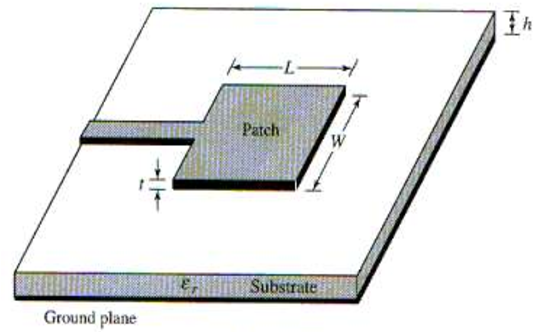
\includegraphics[width=0.5\textwidth]{patch-antenna-structure.png}
    %\end{subfigure}
    \caption{The basic structure of a patch antenna. This particular antenna is being fed with a microstrip. The ground, and the patch are conductors. The substrate is a dielectric. \cite{girase2014design}}
\end{figure}

Besides its large size at lower frequencies, a PA with Figure 1's design would have a narrow frequency band, low efficiency, low power, high Q, poor polarization purity, and spurious feed radiation\cite{balanis2016antenna}. Fortunately, significant effort has gone into addressing these limitations, and a variety of design techniques to mitigate these limitations have been created\cite{balanis2016antenna}. Furthermore, PAs have also been investigated theoretically, and theories to describe the operating mechanism of most PAs have been created. However, the theories describing PA operation are mathematically dense, and are quite challenging to read. This unapproachability in theory leads to obfuscation on both the theory of PA operation, and research associated with it. One of the most intuitive high level ways of describing antennas is visually. While antenna simulation software does exist, it seems like nobody has used it provide a surface level introduction to patch antennas. This paper intends to do so, using the antenna simulation software known as HFSS, by Ansys. HFSS is a 3D electro-magnetic field simulator, used by RF engineers to design antennas, but it can also be used to visualize the fields in patch antennas, thereby giving an intuitive explanation of why certain antenna designs work, and others don't.

This paper will use HFSS to provide a visual explanation of the radiation mechanism of a basic PA, as well as show some of its properties. Afterwards, the paper will review some methods which have been used to miniaturize PAs. None of the presented methods will be exceptionally novel, however, the methods are actually used in current patch antennas, and the mechanism behind their operation is fascinating in its own right. Since this is a surface level paper, certain concepts will be introduced without adequate in depth explanation. In these cases, the paper will reference other readings for a more in depth explanation.            
  
\section{Patch Antenna}

\subsection{Basic Characteristics}
As shown in figure 1, a basic patch antenna consists of a very thin metallic strip (the patch), placed a small fraction of a wavelength above a metallic ground plane. While patches are usually either rectangular or circular\cite{khan2015microstrip}, numerous other shapes have been investigated\cite{balanis2016antenna}. In between the patch, and ground plane, is a dielectric. Dielectrics are electronic insulators which can be polarized by an external electric field. 

\begin{figure}[h]
    %\begin{subfigure}{0.5\textwidth}
    \centering
    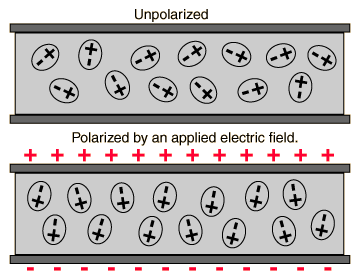
\includegraphics[width=0.3\textwidth]{dielectric.png}
    %\end{subfigure}
    \caption{ [Uncited, provide a citation here] A dielectric with and without an applied E-field. The dielectric constant $\epsilon_r$ (relative permittivity) is a measure of how much the atoms in the dielectric align to the external E-field. Dielectrics with low $\epsilon_r$ will polarize less to the external E-field, compared to high $\epsilon_r$ dielectrics.}
\end{figure}

Numerous dielectric materials are used in PAs. Most of these materials will have dielectric constants in the range of $2.2$ to $12$\cite{balanis2016antenna}. More discussion on the choice of substrate in the antenna will be provided in section 3. 
\subsection{Radiation Mechanism}
There are 3 models used to describe the operation of a patch antenna.
\subsection{Properties}

\section{Substrate Loading}

\newpage
\bibliographystyle{IEEEtran}
\bibliography{main}
%\printbibliography


\end{document}
